\documentclass[9pt,a4paper]{article}

\usepackage[latin1]{inputenc}
\usepackage[cyr]{aeguill}
\usepackage[francais]{babel}

% %\renewcommand{\baselinestretch}{1.5}  % line spacing : 1,5
% \setlength{\oddsidemargin}{2,5cm}	% Marge gauche sur pages impaires
% \setlength{\evensidemargin}{2,5cm}	% Marge gauche sur pages paires
% \setlength{\textwidth}{16cm}	% Largeur de la zone de texte (17cm)
% \setlength{\topmargin}{2,5cm}	% Pas de marge en haut
 
% Les packages
%\usepackage[french]{babel}
\usepackage{fancybox}
\usepackage{graphics}
\usepackage{color}
\usepackage{latexsym}
\usepackage{amsmath,amsthm,amssymb}
\usepackage[T1]{fontenc}
\usepackage[latin1]{inputenc}
\usepackage{fullpage} 
\usepackage{verbatim}
\usepackage{times,epsfig}
\usepackage{listings}
\usepackage{multirow}
\usepackage{amsmath,amsthm,amssymb,amscd,txfonts,bbm} % RAJOUT ICI !!!
\usepackage{graphics,epsfig} % RAJOUT ICI !!!
%\usepackage{algorithmic}
\usepackage[final]{pdfpages} 
\usepackage{fancyvrb}

\newenvironment{qv}
{\quote\Verbatim}
{\endquote\endVerbatim}


\newcommand{\terme}[1]{\texttt{#1}}
\newcommand{\termSet}[1]{\{\texttt{#1}\}}
\newcommand{\guill}[1]{<<\,#1\,>>}
% Macro pour l'inclusion de figure  
\newcommand{\fig}[3]{%
  \begin{figure*}[hbt]
   \begin{center}
      \includegraphics[width=#1]{#2}
  \caption{\label{#2}  #3}
  \end{center}
 \end{figure*}
}
\newcommand{\figTex}[2]{%
  \begin{figure*}[hbt]
 \centerline{\input{#1.pstex_t}}
  \caption{\label{#1}  #2}
 \end{figure*}
}

% Macro commentaires
\definecolor{turquoise}{rgb}{0.20 ,0.60, 0.60}
\definecolor{vert}{rgb}{0.40,  0.60 ,0.00}
\definecolor{violet}{rgb}{0.80 , 0.00 , 0.80}
\definecolor{bleu}{rgb}{0.20,  0.20,  0.80}
\definecolor{rose}{rgb}{1.00,  0.20,  0.40}
\def\remVG#1{\textcolor{vert}{\texttt{Virginie: #1}}}
\def\comVG#1{\begin{footnotesize}\textcolor{vert}{\texttt{Precision de Virginie: #1}}\end{footnotesize}}



\newcommand{\correction}[1]{ ~\newline~ \textcolor{vert}{Correction : #1}}
%\newcommand{\correction}[1]{}

                              
                             
\usepackage{url}

\newtheorem{Exercices}{Definition}

\lstset{language=XML,basicstyle=\footnotesize,
numberstyle=\footnotesize, 
breaklines=true
showspaces=false,         
showstringspaces=false,
showtabs=false,
frame=single,
tabsize=4}   


\begin{document}

\title{CNAM Paris \\ NFE204 - \textit{Bases de donn�es avanc�es (1)} \\ Travaux dirig�s et pratiques \\ XQuery\\
\textcolor{vert}{\textsc{Fichier avec indications de correction}}}

% \author{Virginie Thion}

\date{}

\maketitle

\section{Le cours}
\input{acces_cours}

\section{Exercices}

\subsection{Les livres}
Cet exercice est tr�s inspir� du cours XQuery du W3 Schools.

\subsubsection{Mat�riel}
\noindent Avant toute chose, R�cup�rez le fichier \texttt{books.xml} sur la page Pli@d.\\

Cet ED consiste en la r�daction de requ�tes XQuery permettant d'interroger ce fichier. Pour tester vos requ�tes XQuery, deux solutions s'offrent � vous :
\begin{itemize}
\item (Pas faisable en salle de TP) Installer le logiciel eXist (Syst�me open source de gestion native de
bases de donn�es XML) que vous pouvez t�l�charger sur
\url{http://www.exist-db.org/download.html}. Y cr�er une base de donn�es 
contenant le fichier \texttt{books.xml} et l'interroger (attention � bien choisir votre contexte d'�valuation et � bien pr�fixer vos requ�tes par \texttt{doc('books.xml')}.
\item Installer le logiciel BaseX (Syst�me open source de gestion native de
bases de donn�es XML) que vous pouvez t�l�charger sur
\url{http://www.inf.uni-konstanz.de/dbis/basex/} (prendre le .jar), 
cr�er une base de donn�es � partir du fichier \texttt{books.xml} et l'interrogez  dans la fen�tre intitul�e XQuery.
\end{itemize} 


\subsubsection{Enonc�}

\noindent \`A l'aide de XQuery, formulez les requ�tes suivantes.

\begin{enumerate}
  \item Quels sont tous les titres de livres ? Formuler cette requ�te � l'aide
  de la syntaxe FLWOR et sans FLWOR.
  \correction{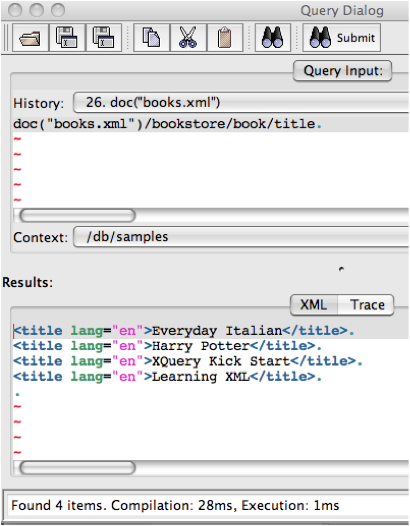
\includegraphics{ED5_XQuery/PourPoly/titres_flowr.png}\\
  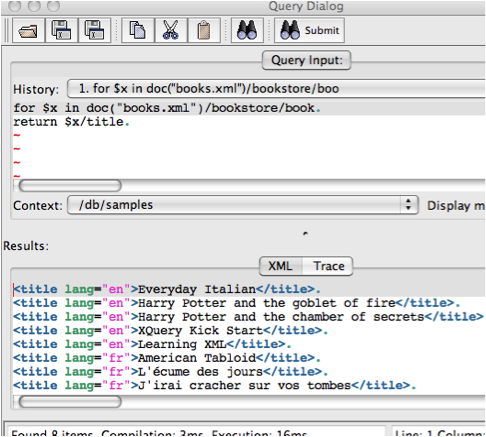
\includegraphics{ED5_XQuery/PourPoly/titres_ss_flowr.png}}
  \item Quels sont tous les livres dont le prix est inf�rieur � 30 ?
  Exprimez cette requ�te de deux fa�ons diff�rentes (l'une grace � une
  expression de chemin et l'autre grace � une requ�te FLWOR).  
  \correction{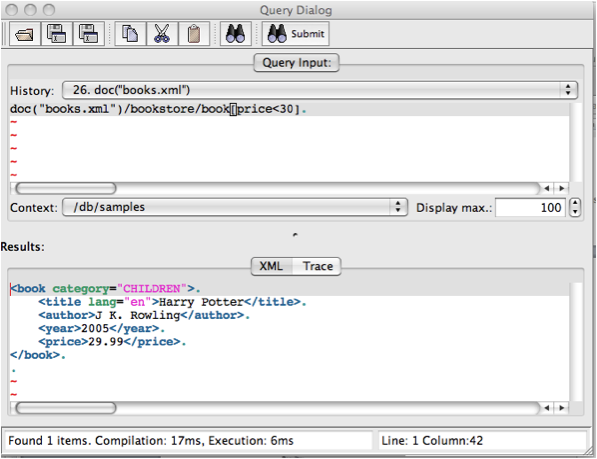
\includegraphics{ED5_XQuery/PourPoly/prix_inf30-1.png}\\
  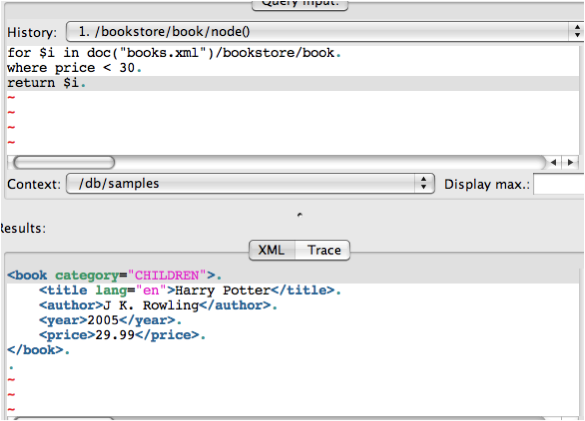
\includegraphics{ED5_XQuery/PourPoly/prix_inf30-2.png}}  
  \item Quels sont les titres des livres dont le prix est inf�rieur � 30 ?
  Formuler cette requ�te � l'aide de la syntaxe FLWOR et sans FLWOR.
  \correction{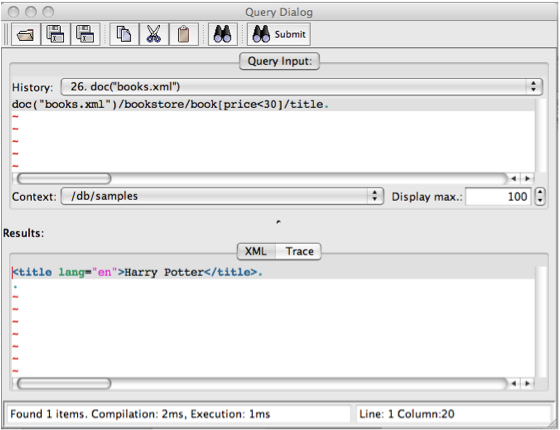
\includegraphics{ED5_XQuery/PourPoly/titre_prix_inf30-1.png}\\
  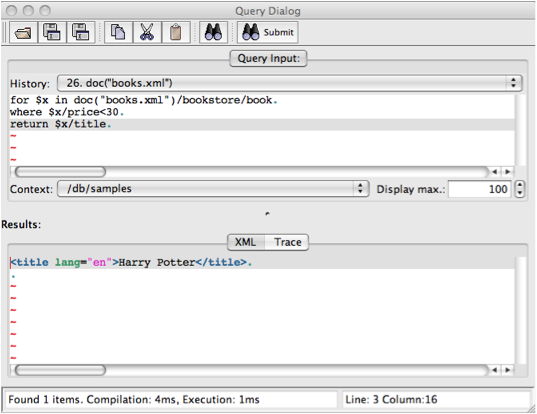
\includegraphics{ED5_XQuery/PourPoly/titre_prix_inf30-2.png}}  
  \item Quels sont les titres des livres dont le prix est sup�rieur � 30,
  ordonn�s par ordre alphab�tique ?
  \correction{\\ for \$x in doc("books.xml")/bookstore/book\\
where \$x/price>30\\
order by \$x/title\\
return \$x/title}
\item Lister les auteurs de livres par ordre alphab�tique.
\correction{Rajouter order by \$author en ligne 2}
\item Lister les livres par date de sortie.
\correction{\\ for \$x in doc("books.xml")/bookstore/book\\
order by \$x/year\\
return \$x}
\item Pr�senter les titres de livres tri�s par ordre alphab�tique dans une
liste XHTML\\ (<ul><li>titre 1</li><li>titre 2</li> ... </ul>)
\correction{\lstinputlisting{ED5_XQuery/PourPoly/reqtitreshtml.xq}}
\item Idem que 7 en �liminant la balise \texttt{<titre>} de la pr�sentation en
utilisant la fonction \texttt{data(e)} qui extrait le texte d'un �l�ment
\texttt{e}.
\correction{\lstinputlisting{ED5_XQuery/PourPoly/reqtitreshtml-2.xq}}
\item En fonction de la cat�gorie des films, produire de nouveaux tags permettant
d'obtenir le r�sultat suivant :
\begin{lstlisting}
<adult>Everyday Italian</adult>
<child>Harry Potter</child>
<adult>Learning XML</adult>
<adult>XQuery Kick Start</adult>
\end{lstlisting}
Ici, les livres dont l'attribut \texttt{category} a pour valeur CHILDREN sont dans un �l�ment \texttt{child} et les livres pour lesquels l'attribut  \texttt{category} a une autre valeur sont dans un �l�ment \texttt{adult}.
\correction{\lstinputlisting{ED5_XQuery/PourPoly/newtag.xq}}
\item Utilisez XQuery pour produire le texte suivant � partir du fichier
books.xml (NB : les livres sont tri�s par ordre alphab�tique).
\begin{lstlisting}
<html>
<body>

<h1>Bookstore</h1>

<ul>
<li>Everyday Italian. Category: COOKING</li>
<li>Harry Potter. Category: CHILDREN</li>
<li>Learning XML. Category: WEB</li>
<li>XQuery Kick Start. Category: WEB</li>
</ul>

</body>
</html>

\end{lstlisting}
\correction{\lstinputlisting{ED5_XQuery/PourPoly/text_livres_alpha.xq}}
 
 \item M�me question. NB : la valeur d'un attribut peut �tre r�cup�r�e en utilisant la fonction \texttt{data} prenant en argument le chemin d'acc�s (au sens XPath) � l'attribut.
 \begin{lstlisting}
<html>
<body>
<h1>Bookstore</h1>

<ul>
<li class="COOKING">Everyday Italian</li>
<li class="CHILDREN">Harry Potter</li>
<li class="WEB">Learning XML</li>
<li class="WEB">XQuery Kick Start</li>
</ul>

</body>
</html>

\end{lstlisting}
\correction{\lstinputlisting{ED5_XQuery/PourPoly/text_livres_alpha-2.xq}} 

\item Lister les auteurs des livres (sans doublon). Rappel : la fonction  \texttt{distinct-values} appliqu�e � une s�quence de {\it valeurs} renvoie la s�quence d�doublonn�e.
\correction{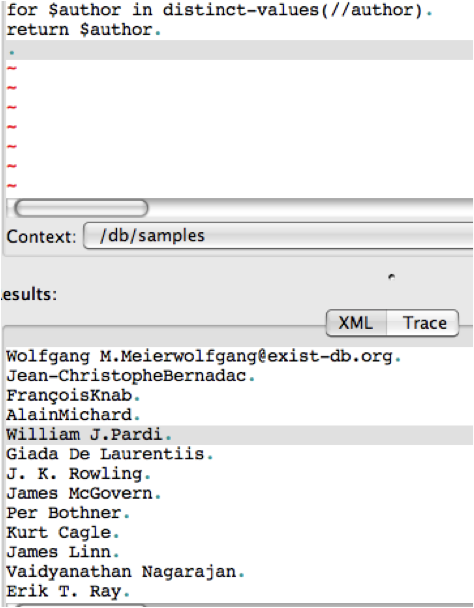
\includegraphics{ED5_XQuery/PourPoly/liste_auteurs.png}. On peut mettre \texttt{data(//author)} pour extraire une sequence de chaine de la s�quence d'�l�ments \texttt{author}, mais \texttt{distinct-values} le fait par d�faut puis qu'il d�doublonne forc�ment sur des s�quences de valeurs (et non des s�quences d'�l�ments).}

\item Utilisez la clause \texttt{for} et un compteur pour produire le r�sultat
suivant :
 \begin{lstlisting}
<book>1. Everyday Italian</book>
<book>2. Harry Potter</book>
<book>3. XQuery Kick Start</book>
<book>4. Learning XML</book>
\end{lstlisting}
\correction{\lstinputlisting{ED5_XQuery/PourPoly/result1.xq}}

\item Jointure. Cr�ez deux fichiers XML de votre choix propices � une jointure.
Effectuer cette jointure � l'aide d'une requ�te XQuery.

\item Quels sont les titres de livres pour lesquels l'un des auteurs a pour pr�nom ou nom ``James'' ?
\correction{\lstinputlisting{ED5_XQuery/PourPoly/james.xq}}

\item Quels sont les titres de livres pour lesquels les auteurs sont
\textit{Vian} ou \textit{Pestureau} (l'un des deux ou les deux) ?
\correction{\lstinputlisting{ED5_XQuery/PourPoly/vian.xq}}
 
\end{enumerate}

\end{document}
